\documentclass{beamer}

\usepackage{pgf}  
\usepackage{tikz}
\usetikzlibrary{arrows}
\usepgflibrary{shapes.arrows} 
\usetikzlibrary{intersections}
\usetikzlibrary{calc}
\usetikzlibrary{fit}
\usetikzlibrary{automata,positioning}
\usepackage{pgfplots,stackengine}
\usepackage{fontspec}
\usepackage{fancyvrb}
\usepackage{wasysym}
\usepackage{unicode-math}
\usepackage{import}
\usepackage{rotating}
\usepackage{gensymb}
\usepackage{chemfig}
\usepackage{rotating}
\usepackage{booktabs}
\usepackage{pifont}
\usepackage{wrapfig}
\usepackage{mathtools}
\usepackage{graphbox}
\usepackage{epigraph}
\usepackage{listings}
\usepackage{verbatim}
\usepackage[absolute,overlay]{textpos}
\usepackage[euler-digits,euler-hat-accent]{eulervm}
%\logo{\pgfputat{\pgfxy(.45,.5)}{\pgfbox[center]{
\includegraphics[width=1.7cm]{Figures/uu_shadow.pngu}}}}

\usetheme{Copenhagen}
\usecolortheme{beaver}

\setbeamercolor{block title}{use=structure,fg=white,bg=red!75!black}
\setbeamercolor*{item}{fg=red}

\newcommand{\unilogo}{
  \setlength{\TPHorizModule}{1pt}
  \setlength{\TPVertModule}{1pt}
  \begin{textblock}{1}(26,-10)
   
\includegraphics[height=70pt, align=c]{Figures/uu_shadow.png}
  \end{textblock}
  } 

\pgfmathdeclarefunction{gauss}{2}{%
  \pgfmathparse{1/(#2*sqrt(2*pi))*exp(-((x-#1)^2)/(2*#2^2))}%
}
  
\makeatletter
    \newcases{mycases}{\quad}{%
        \hfil$\m@th\displaystyle{##}$}{$\m@th\displaystyle{##}$\hfil}{\lbrace}{.}
\makeatother

\addtobeamertemplate{frametitle}{}{%
    \unilogo
}
\setlength{\fboxsep}{0pt}

\begin{document}
\graphicspath{{Figures/}}
\setsansfont[ItalicFont = Optima Italic,
             BoldFont = Optima Bold,
             Ligatures=TeX ]
            {Optima Regular}
\setmainfont[ItalicFont = Optima Italic,
             BoldFont = Optima Bold,
             Ligatures=TeX]
            {Optima Regular}
\newfontfamily\commentfont[]{Chalkboard}
\newcommand{\lmr}{\fontfamily{lmr}\selectfont}
\newfontfamily\zA[Ligatures={Common, Rare}, Variant=1] {Zapfino}
\newfontfamily\zB[Ligatures={Common, Rare}, Variant=2] {Zapfino}
\newfontfamily\zC[Ligatures={Common, Rare}, Variant=3] {Zapfino}
\newfontfamily\zD[Ligatures={Common, Rare}, Variant=4] {Zapfino}
\newfontfamily\zE[Ligatures={Common, Rare}, Variant=5] {Zapfino}
\newfontfamily\zF[Ligatures={Common, Rare}, Variant=6] {Zapfino}
\newfontfamily\zG[Ligatures={Common, Rare}, Variant=7] {Zapfino}
\renewcommand\UrlFont{\color{blue}}
\definecolor{uured}{RGB}{153,0,0}

\title{{\lmr \LaTeX}}   
\author{Jonathan Alvarsson} 
%\titlegraphic{\vfill\includegraphics[width=18em]{Figures/ORN_large.png}}
\date{April 2020} 

\setbeamertemplate{background}{%
    \parbox[c][\paperheight]{\paperwidth}{%
        \vfill
        \hfill
        
\includegraphics[height=0.65\textheight]{Figures/sigill.png}
    }   
}
\begin{frame}[plain]
\unilogo\titlepage
\begin{tikzpicture}[remember picture,overlay]
\tikz[remember picture, overlay] \fill[uured] (current page.north west) rectangle ++(\paperwidth,-0.5cm);
\end{tikzpicture}%
\end{frame}

\setbeamertemplate{background}{}
\renewcommand{\unilogo}{
  \setlength{\TPHorizModule}{1pt}
  \setlength{\TPVertModule}{1pt}
  \begin{textblock}{1}(0,0)
   
\includegraphics[height=27pt, align=c]{Figures/uu.png}
  \end{textblock}
  } 
\section{Background}
    \begin{frame}
    \frametitle{Outline}
    \begin{minipage}{0.25\textwidth}
    \mbox{}
    \end{minipage}
    \begin{minipage}{0.6\textwidth}
    \tableofcontents[hideallsubsections]
    \end{minipage}
    \end{frame}
    \subsection{What is {\lmr \LaTeX}?}
    \begin{frame}
        \frametitle{Background}
        \framesubtitle{What is {\lmr \LaTeX}?}
        \begin{block}{{\lmr \LaTeX} and {\lmr \TeX}}
        {\lmr \LaTeX} is a \alert{document preparation system} based on the
        {\lmr \TeX} typesetting system. {\lmr \TeX} was written by Donald Knuth
        roughly between the years 1977 and 1989. {\lmr \LaTeX}
        was created in the early 1980s by Leslie Lamport.
        \end{block}
    \end{frame}
    \begin{frame}[fragile]
        \frametitle{Background}
        \framesubtitle{What is {\lmr \LaTeX}?}

            \lstset{language=Tex, }
\begin{lstlisting}
\documentclass{article}
\begin{document}
\section*{Part 1}
A small example. \LaTeX is often used for math:
\begin{equation}
    y = \frac{1}{x}
\end{equation}
\section*{Part 2}
\end{document}
\end{lstlisting}
        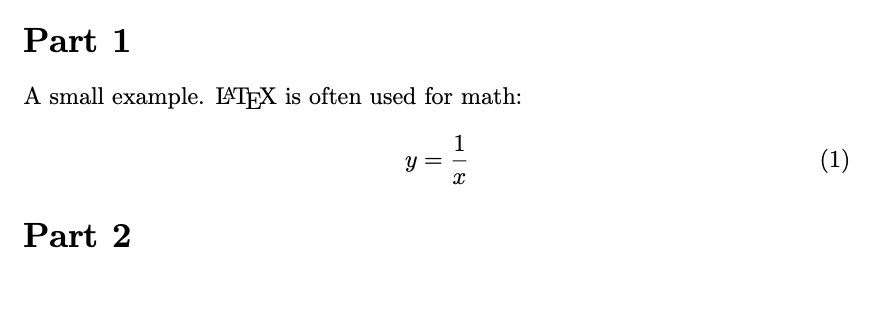
\includegraphics[width=0.5\textwidth]{figures/formath.png}
    \end{frame}

    \section{Workflows}
    \subsection{Vim + latexmk + Skim}
    \begin{frame}
        \frametitle{Vim + latexmk + Skim}
        \framesubtitle{I prefer to write in Vim}
        \fbox{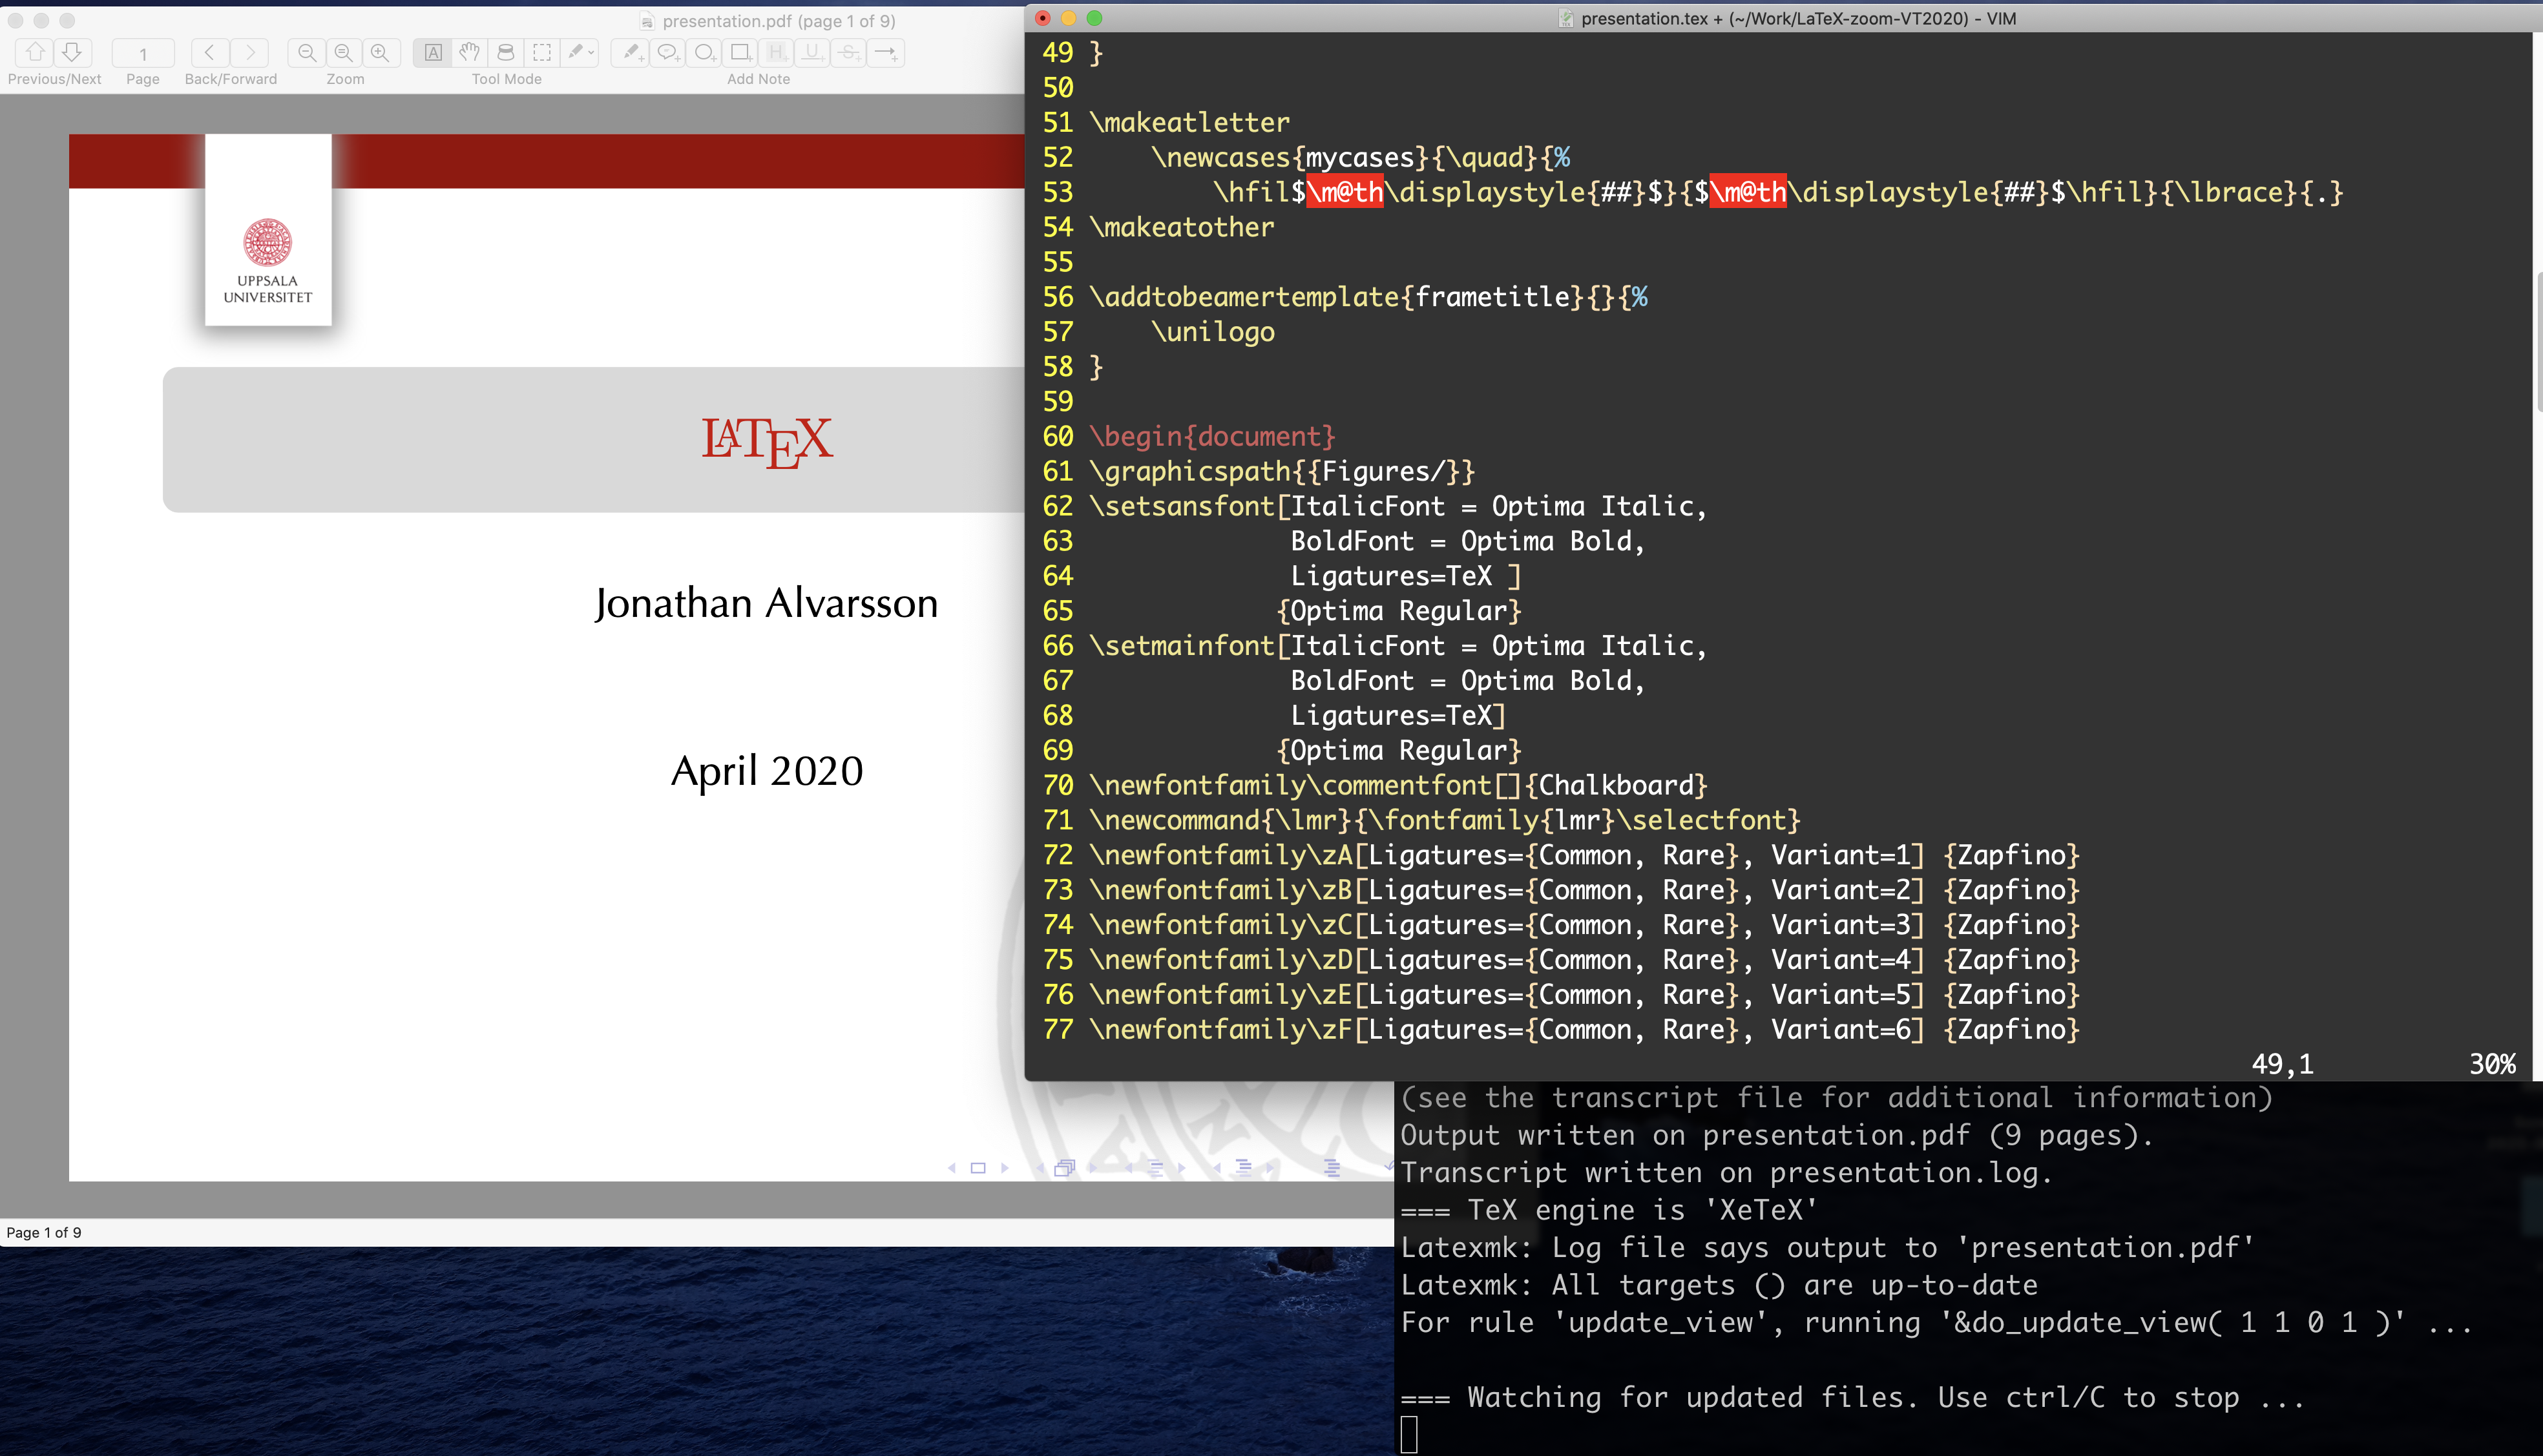
\includegraphics[width=1\textwidth]{figures/vim.png}}
    \end{frame}
    \subsection{Texshop}
    \begin{frame}
        \frametitle{Texshop}
        \framesubtitle{Texshop is a Mac program for typesetting using {\lmr \LaTeX}}
        \fbox{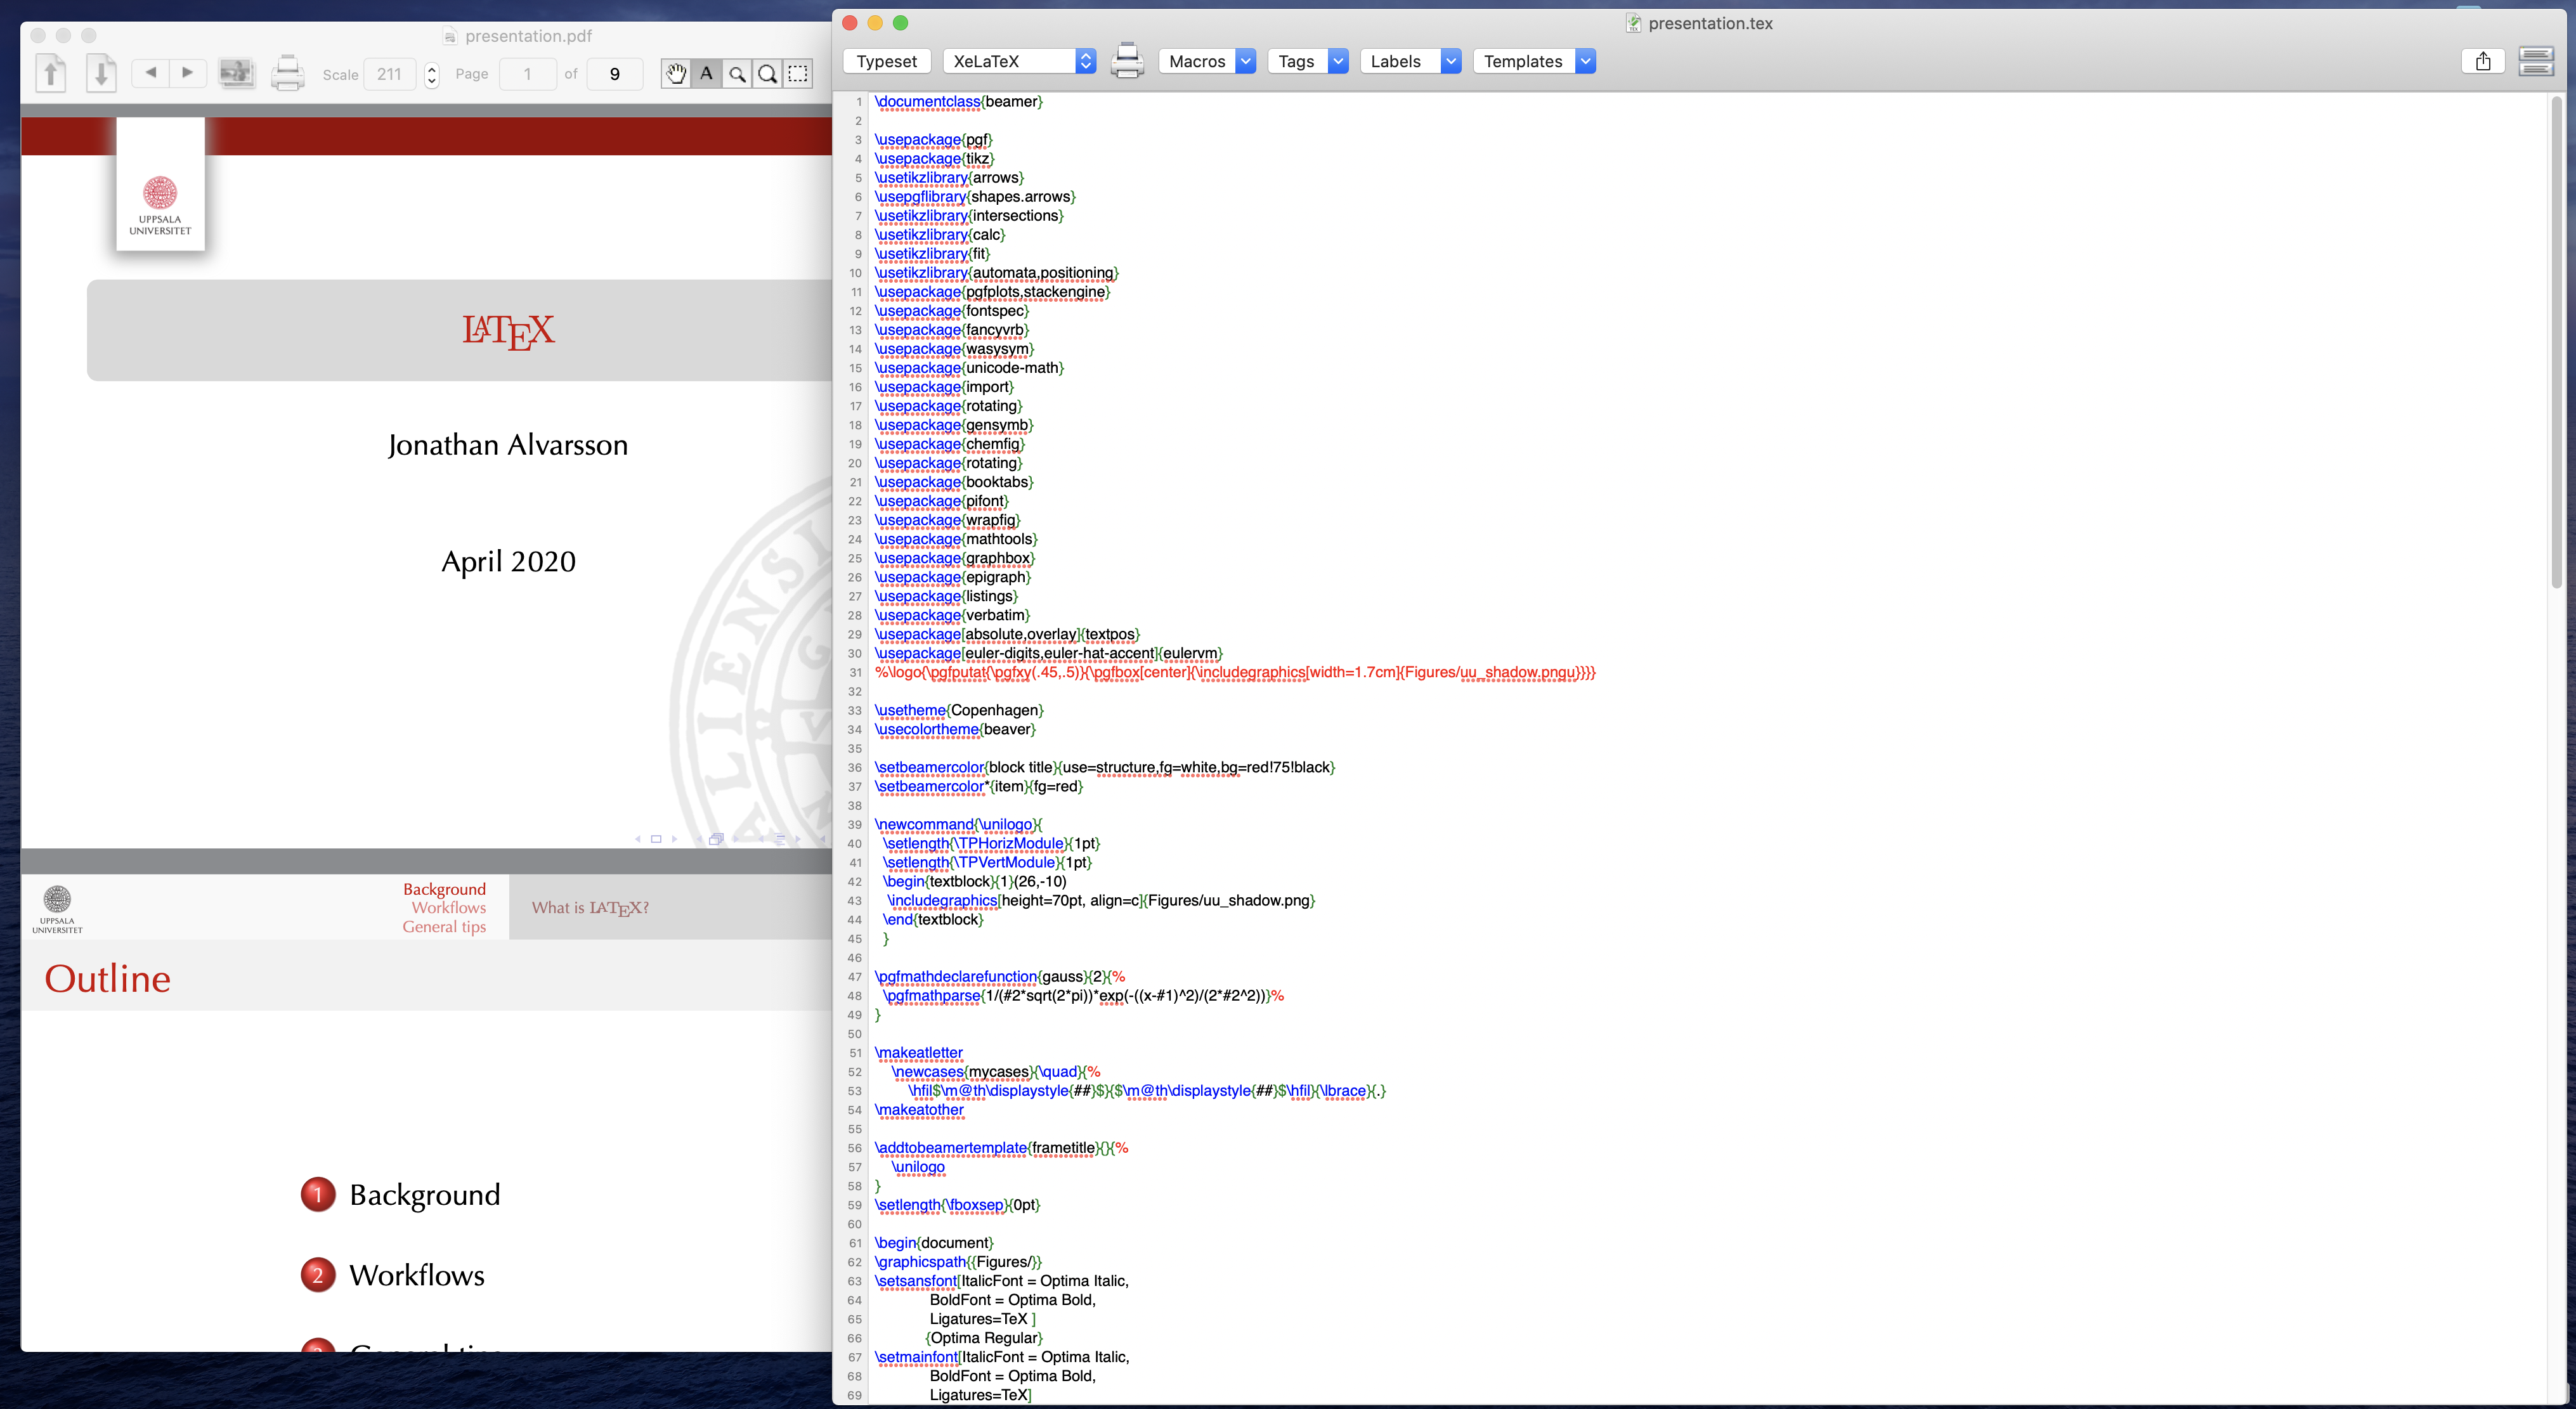
\includegraphics[width=1\textwidth]{figures/texshop.png}}
    \end{frame}
    \subsection{Overleaf}
    \begin{frame}
        \frametitle{Overleaf}
        \framesubtitle{Overleaf is an online solution with good and bad things}
        \centering
        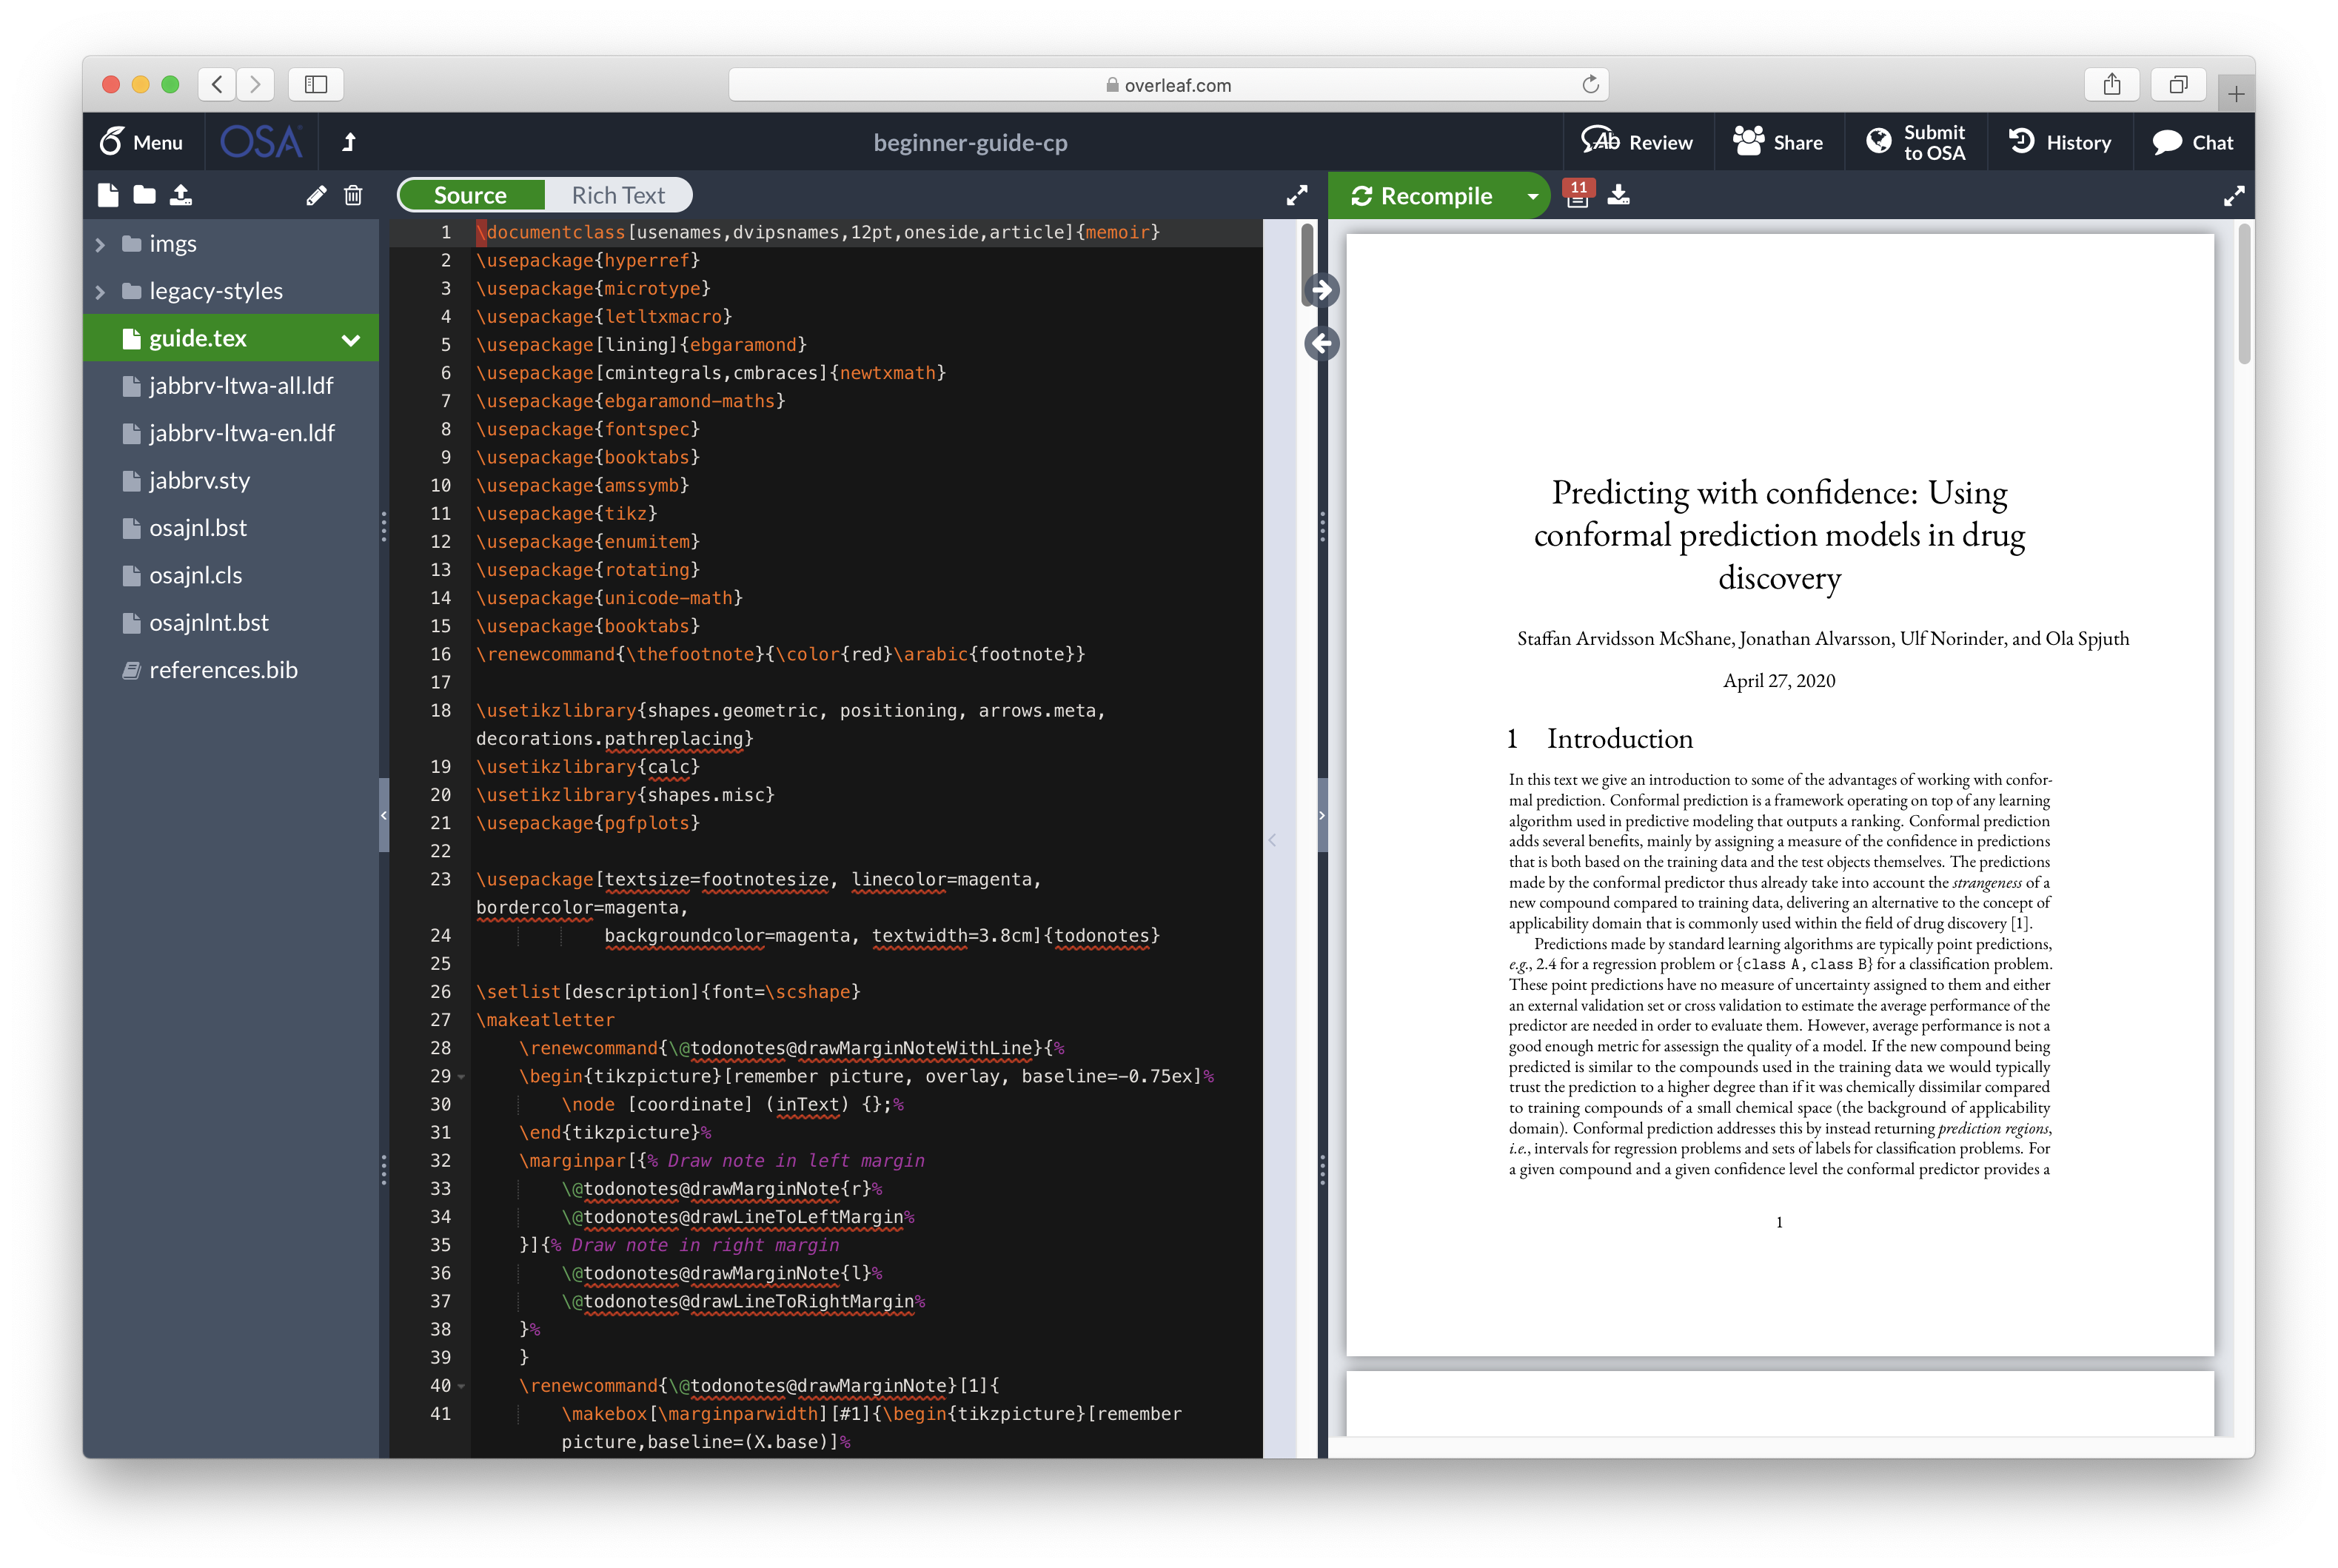
\includegraphics[width=0.95\textwidth]{figures/overleaf.png}
    \end{frame}
    \section{General tips}
    \begin{frame}
    \end{frame}

    \setbeamertemplate{background}{%
        \parbox[c][\paperheight]{\paperwidth}{%
            \vskip -14 ex \hskip -5 em
            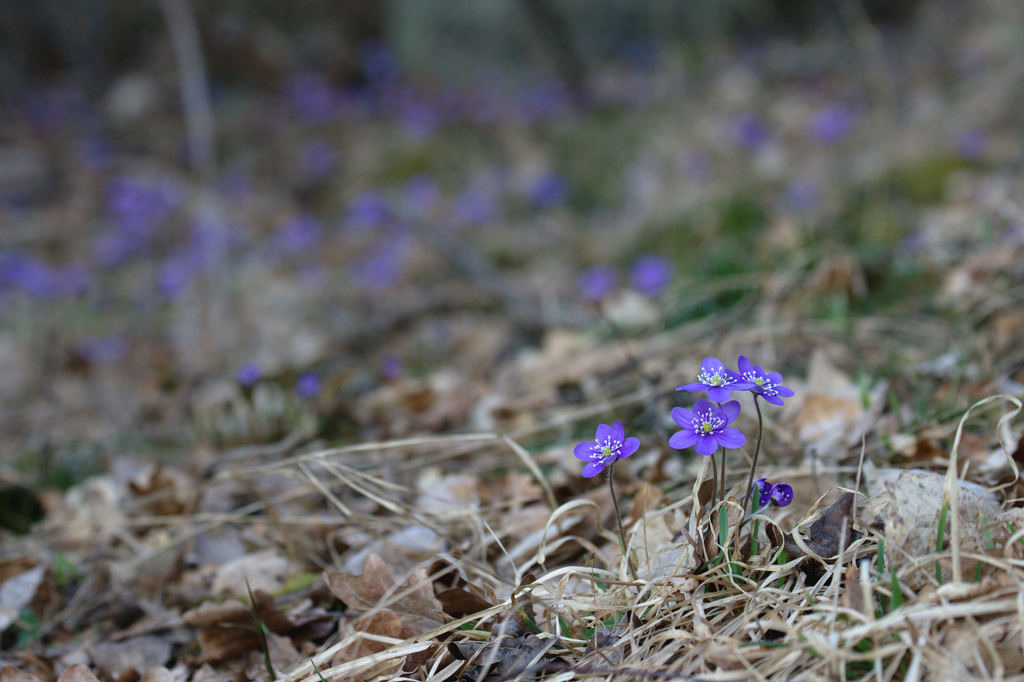
\includegraphics[height=1.275\paperheight]{Figures/blasippa.jpg}
        }   
    }
    \begin{frame}[plain]
        \vfill{\Huge\qquad\color{white} \zB Thank \zC you}\vfill
    \end{frame}
    \setbeamertemplate{background}{}
\end{document}
